

\begin{table}
	\centering
	\caption{Best-fit parameters with $1\sigma$ credibility intervals for all sets of models.}
	\begin{tabular}{l l l l}

		\hline
		Parameter                 & Value                                                                    \\
		\hline
		$f_b$                     & $0\%$                  & $2\%$                  & $10\%$                 \\
		$W_0$                  & $6.26^{+0.10}_{-0.10}$ & $6.28^{+0.10}_{-0.10}$ & $6.36^{+0.09}_{-0.09}$ \\
		$M/10^6 \mathrm{M}_\odot$ & $0.88^{+0.01}_{-0.01}$ & $0.89^{+0.01}_{-0.01}$ & $0.89^{+0.01}_{-0.01}$ \\
		$r_h / pc$                & $6.72^{+0.06}_{-0.06}$ & $6.74^{+0.06}_{-0.06}$ & $6.77^{+0.06}_{-0.06}$ \\
		$\log_{10}{r_a / pc}$     & $1.51^{+0.07}_{-0.05}$ & $1.50^{+0.06}_{-0.05}$ & $1.48^{+0.06}_{-0.05}$ \\
		$g$                       & $1.37^{+0.06}_{-0.06}$ & $1.36^{+0.06}_{-0.06}$ & $1.34^{+0.06}_{-0.06}$ \\
		$\delta$                  & $0.43^{+0.02}_{-0.02}$ & $0.43^{+0.02}_{-0.02}$ & $0.41^{+0.01}_{-0.01}$ \\
		$s^2$                     & $0.01^{+0.01}_{-0.00}$ & $0.01^{+0.01}_{-0.00}$ & $0.01^{+0.01}_{-0.00}$ \\
		$F$                       & $3.26^{+0.13}_{-0.12}$ & $3.24^{+0.13}_{-0.12}$ & $3.16^{+0.13}_{-0.12}$ \\
		$\alpha_1$                & $0.35^{+0.02}_{-0.02}$ & $0.37^{+0.02}_{-0.02}$ & $0.45^{+0.02}_{-0.02}$ \\
		$\alpha_2$                & $1.46^{+0.05}_{-0.05}$ & $1.47^{+0.05}_{-0.05}$ & $1.53^{+0.05}_{-0.04}$ \\
		$\alpha_3$                & $2.13^{+0.04}_{-0.03}$ & $2.18^{+0.04}_{-0.04}$ & $2.46^{+0.05}_{-0.05}$ \\
		$BH_{ret} (\%)$           & $0.07^{+0.06}_{-0.05}$ & $0.08^{+0.09}_{-0.05}$ & $0.17^{+0.18}_{-0.12}$ \\
		$d$                       & $4.42^{+0.02}_{-0.02}$ & $4.42^{+0.02}_{-0.02}$ & $4.43^{+0.02}_{-0.02}$ \\
		\hline
	\end{tabular}
	\label{tab:parameters_all}
\end{table}







In each set of models, all observables are very well reproduced, showing the flexibility of the
\code{LIMEPY} models. Due to this flexibility, it is unlikely that with current observations we
would be able to infer anything about the binary population of a cluster using this technique.
Instead, this method should be used in cases where there are existing estimates of the binary
population within a cluster in order to add a realistic binary component to \code{LIMEPY} models



\section{The Effects of the Binaries}


Table \ref{tab:parameters_all} shows the recovered parameters for each set of models. We can see a
clear agreement in the recovered values of the parameters which affect the overall structure of the
cluster. In particular, the total cluster mass, half-mass radius, anisotropy radius, truncation
parameter, degree of mass segregation and distance are all either identical or within $1\sigma$ of
each other for all three sets of models.



The most striking change in model parameters are the values pertaining to the mass function, in
particular, the $\alpha_3$ parameter which controls the slope of the high-mass mass function (above
$1.0 \ \mathrm{M}_\odot$). In the case with a $10\%$ binary fraction, this parameter is much larger
than in the other two cases showing that the abundance of binary stars reduces the need for high-mass
stars and remnants.

We can see that there is still some need for black holes in some of the models with a high binary fraction
as the $BH_{ret}$ parameter is much larger in the model with many binaries, this means that even
though the initial mass function produces many fewer black holes, more of these black holes need to
be retained throughout the evolution of the cluster.

Table \ref{tab:BH_contents} and Figure \ref{fig:BH_KDEs} show the distribution of BHs for each set
of models. We can see a clear decrease in the inferred black hole content as we add more binaries
though we also note that all three sets of models are consistent with zero black holes within their
$2\sigma$ intervals. This effect of binaries reducing the need for black holes was also found by
\citet{Mann2019} (see also associated erratum \citealt{Mann2020}) when they modelled the central
kinematics of 47\,Tuc. This effect is due to the high-mass binary systems which have mass-segregated
to the central regions of the cluster contributing to the central mass distribution in a similar way
to heavy stellar remnants. Through this process, fewer black holes are needed to create the observed
central velocity dispersion. This effect is particularly clear in Figure \ref{fig:mass_enc_comp}
where we examine the enclosed mass profiles of remnants and binaries for the no-binary and
high-binary cases.



\begin{figure}
	\centering
	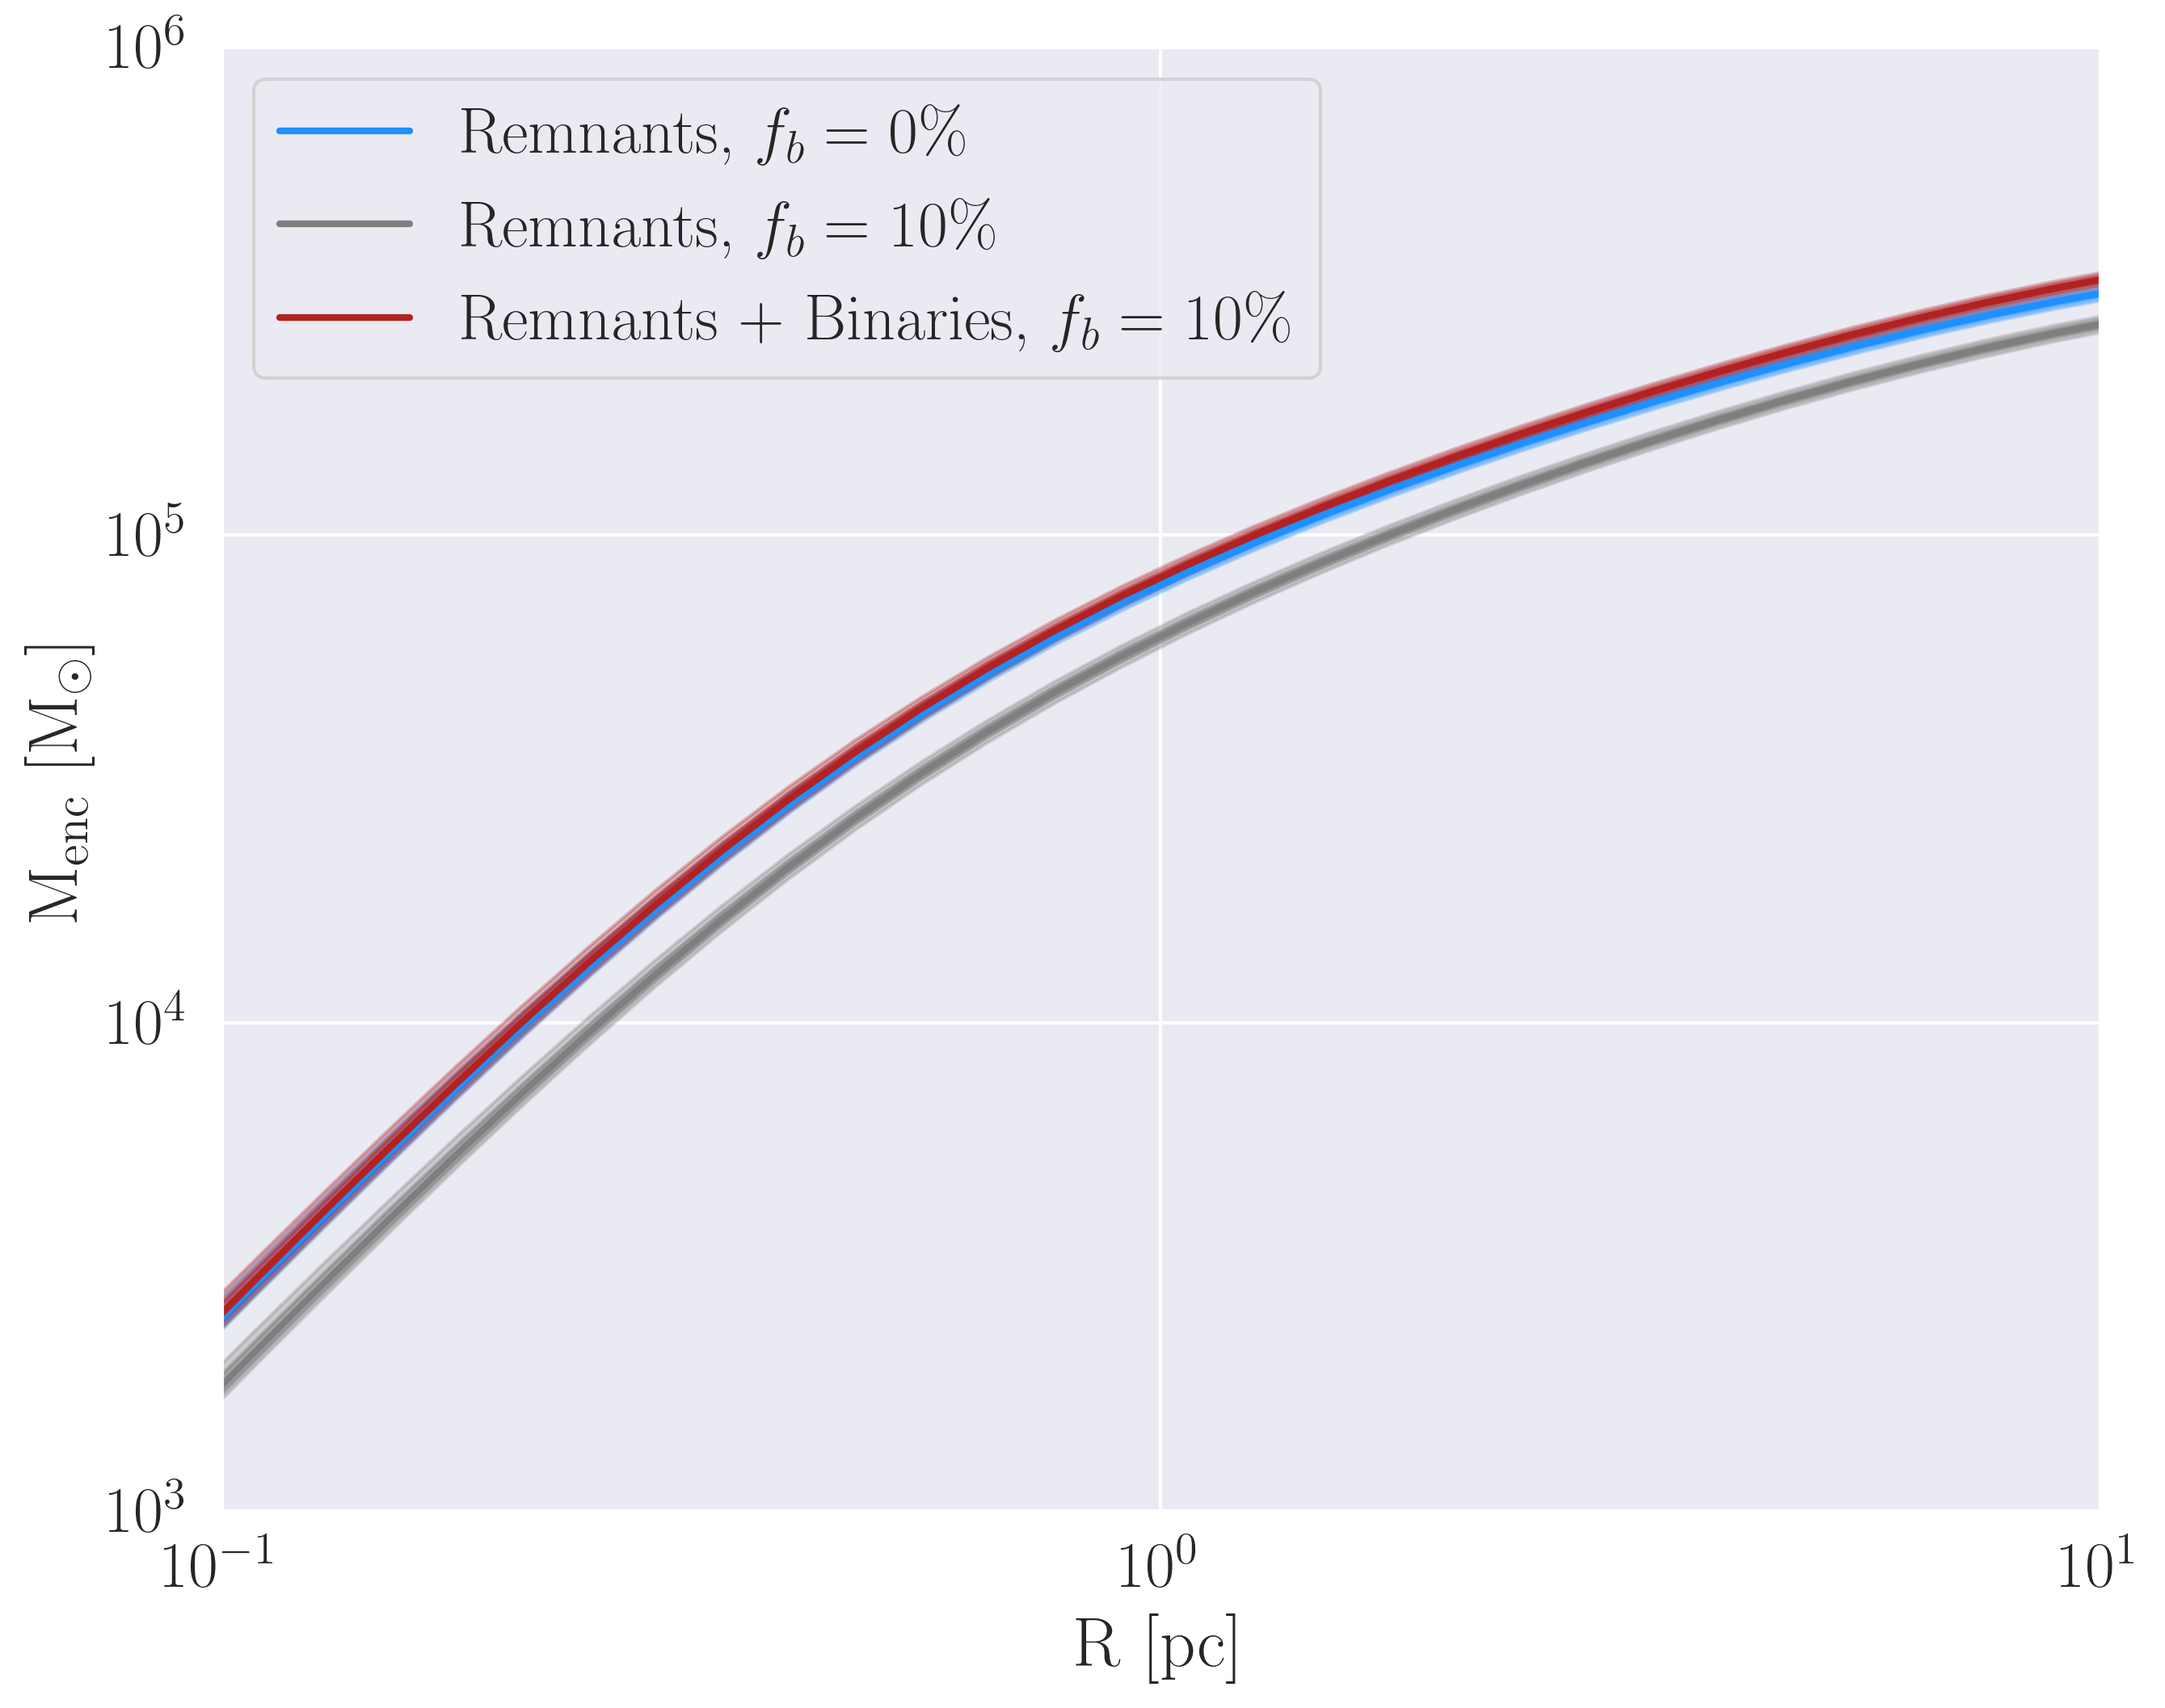
\includegraphics[width=0.8\textwidth]{figures/mass_enc_comp.png}
	\caption{Enclosed mass profiles for the stellar remnants in the $f_b =0\%$ model and the
		remnants and remnants plus binaries in the $f_b =10\%$ model. The two remnant
		profiles are very different between the $f_b = 0\%$ and $f_b = 10\%$ cases which
		mirrors the lower black hole content. The most interesting part of these profiles is
		the fact that when the \emph{binaries} are added to the remnants the enclosed mass
		profiles match very well. This demonstrates very clearly that the binaries are
		filling the same role as the heavy remnants in the central regions of the cluster
		and explains why adding binaries reduces the need for black holes in the models.}
	\label{fig:mass_enc_comp}
\end{figure}


% Table comparing bh content in each set of models
\begin{table}
	\centering
	\caption{Black hole content in each set of models}
	\begin{tabular}{c c c}
		\hline
		Binary Fraction $(\%)$ & Mass in BHs                         & Number of BHs    \\
		\hline
		0                      & $136^{+108}_{-91} \mathrm{M}_\odot$ & $26^{+15}_{-15}$ \\
		2                      & $114^{+144}_{-79} \mathrm{M}_\odot$ & $22^{+19}_{-13}$ \\
		10                     & $81 ^{+121}_{-81} \mathrm{M}_\odot$ & $12^{+13}_{-12}$ \\
		\hline
	\end{tabular}
	\label{tab:BH_contents}
\end{table}


\begin{figure}
	\centering
	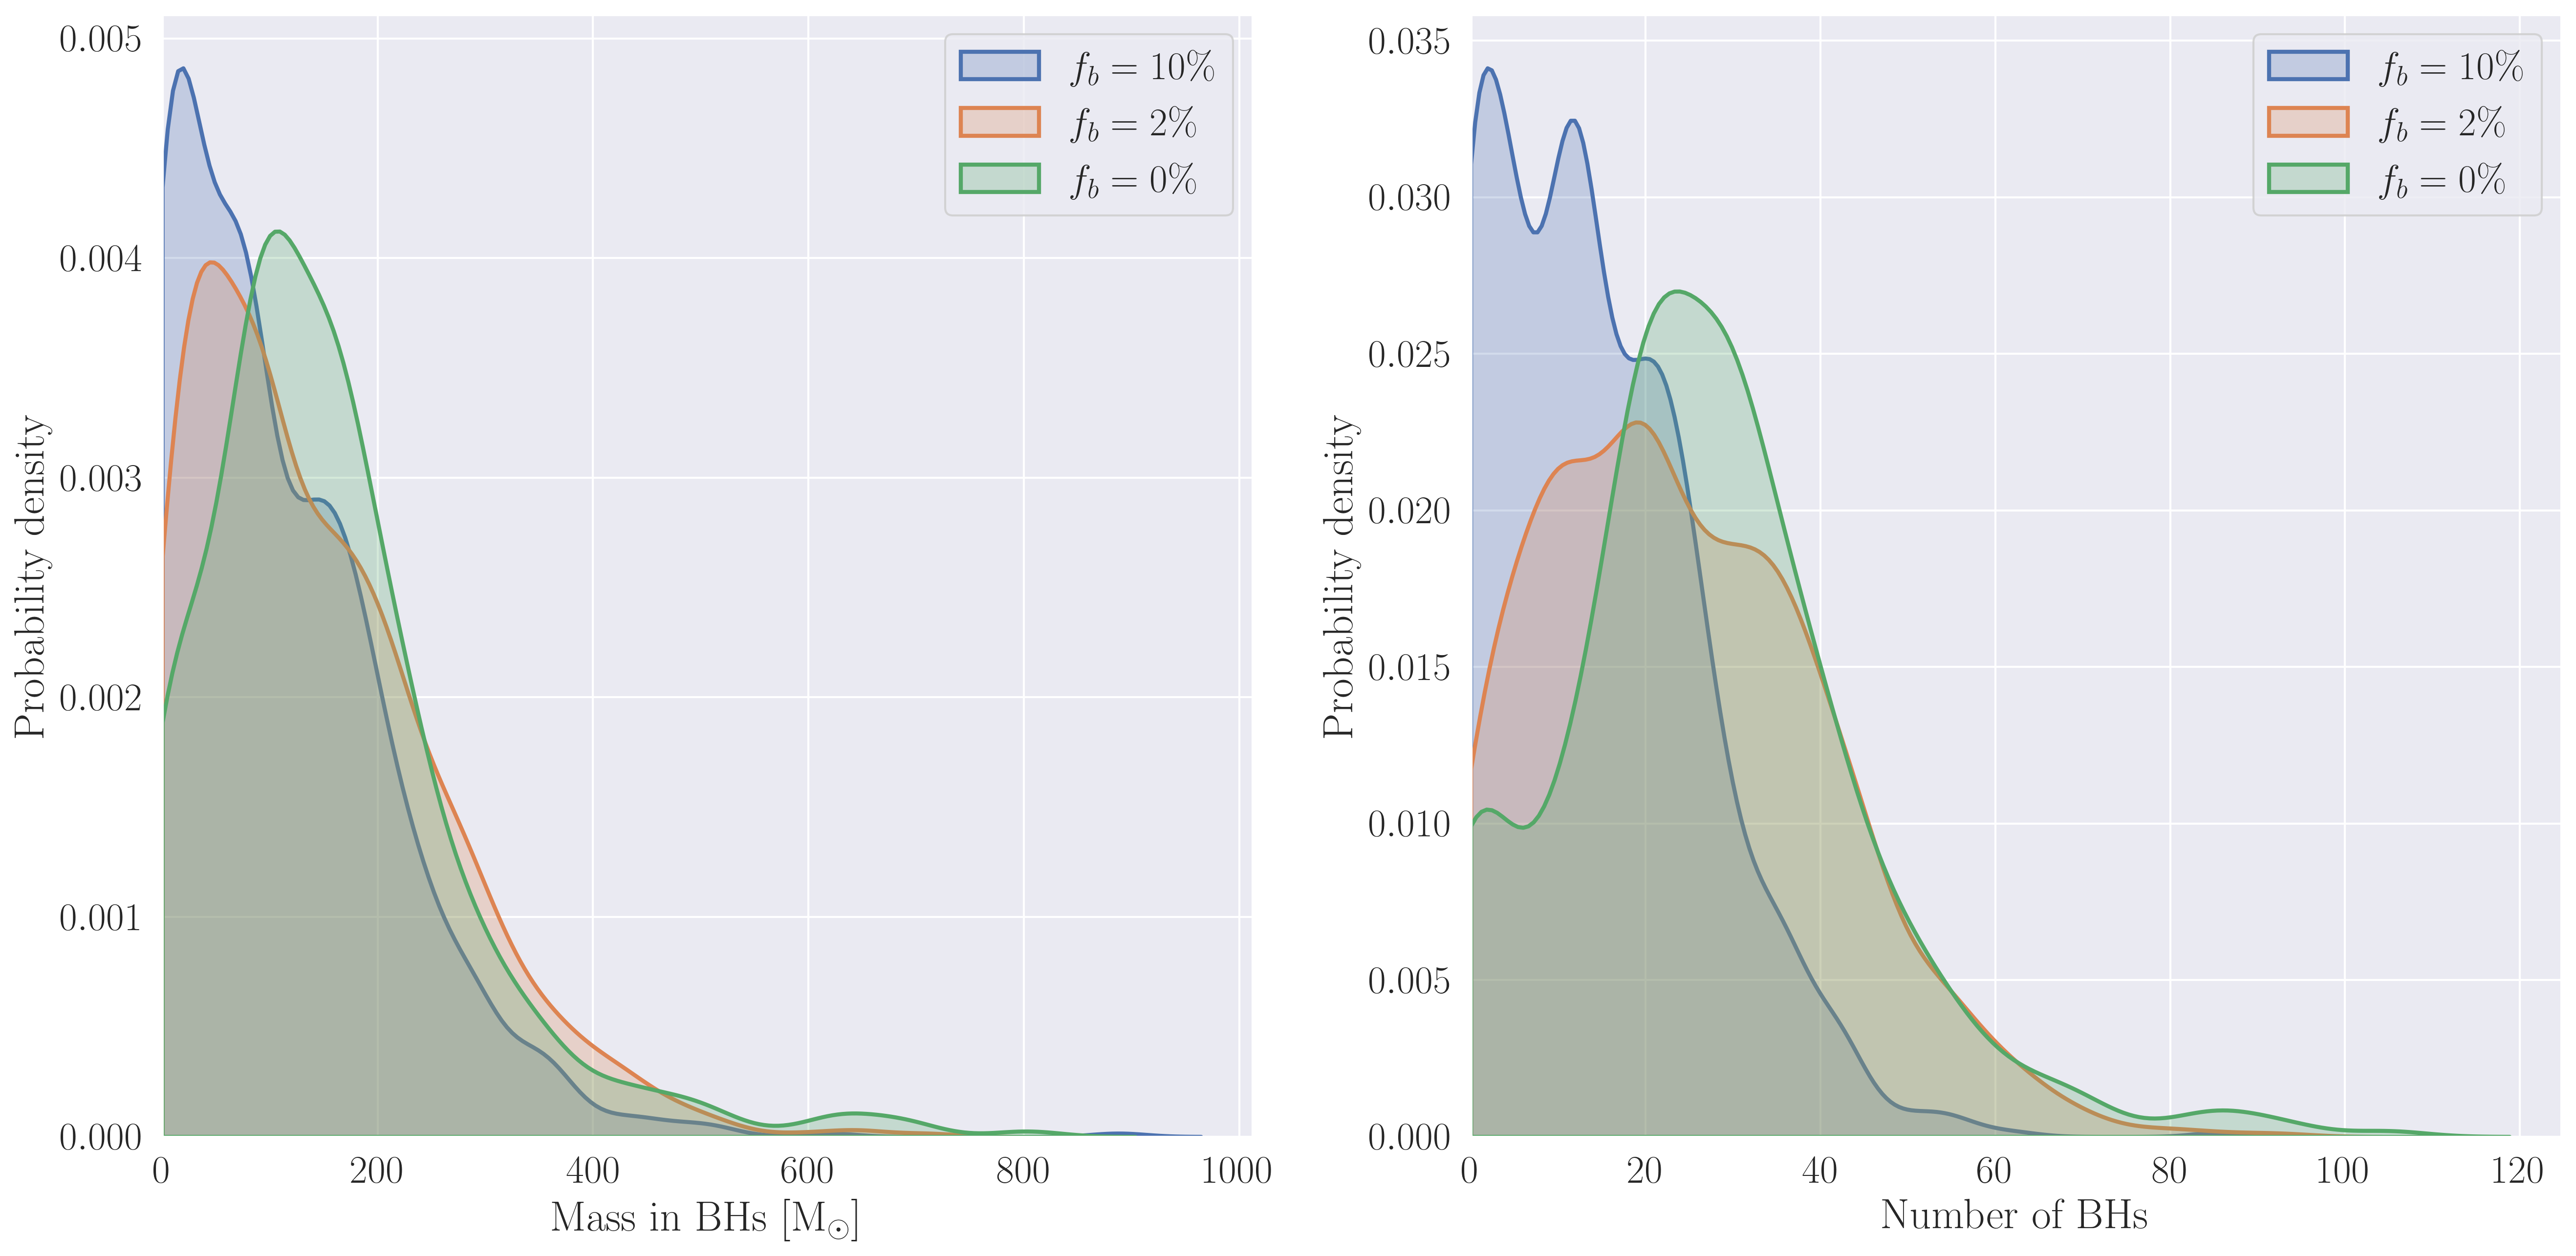
\includegraphics[width=\textwidth]{figures/BH_KDEs.png}
	\caption{Distribution of mass and number of BHs in each set of models. Distributions are
		represented by a Gaussian kernel density estimator of the discrete values for easier visual
		comparison.}
	\label{fig:BH_KDEs}
\end{figure}

When we examine the density profiles for the models with a binary fraction of $10\%$ (see Figure
\ref{fig:highbin_model_densities}), we can see that the binary stars are indeed more centrally
concentrated than typical main-sequence stars as predicted and in the central regions, make up
almost all the main-sequence contribution, while they contribute more than the neutron stars at all
radii.



\begin{figure}
	\centering
	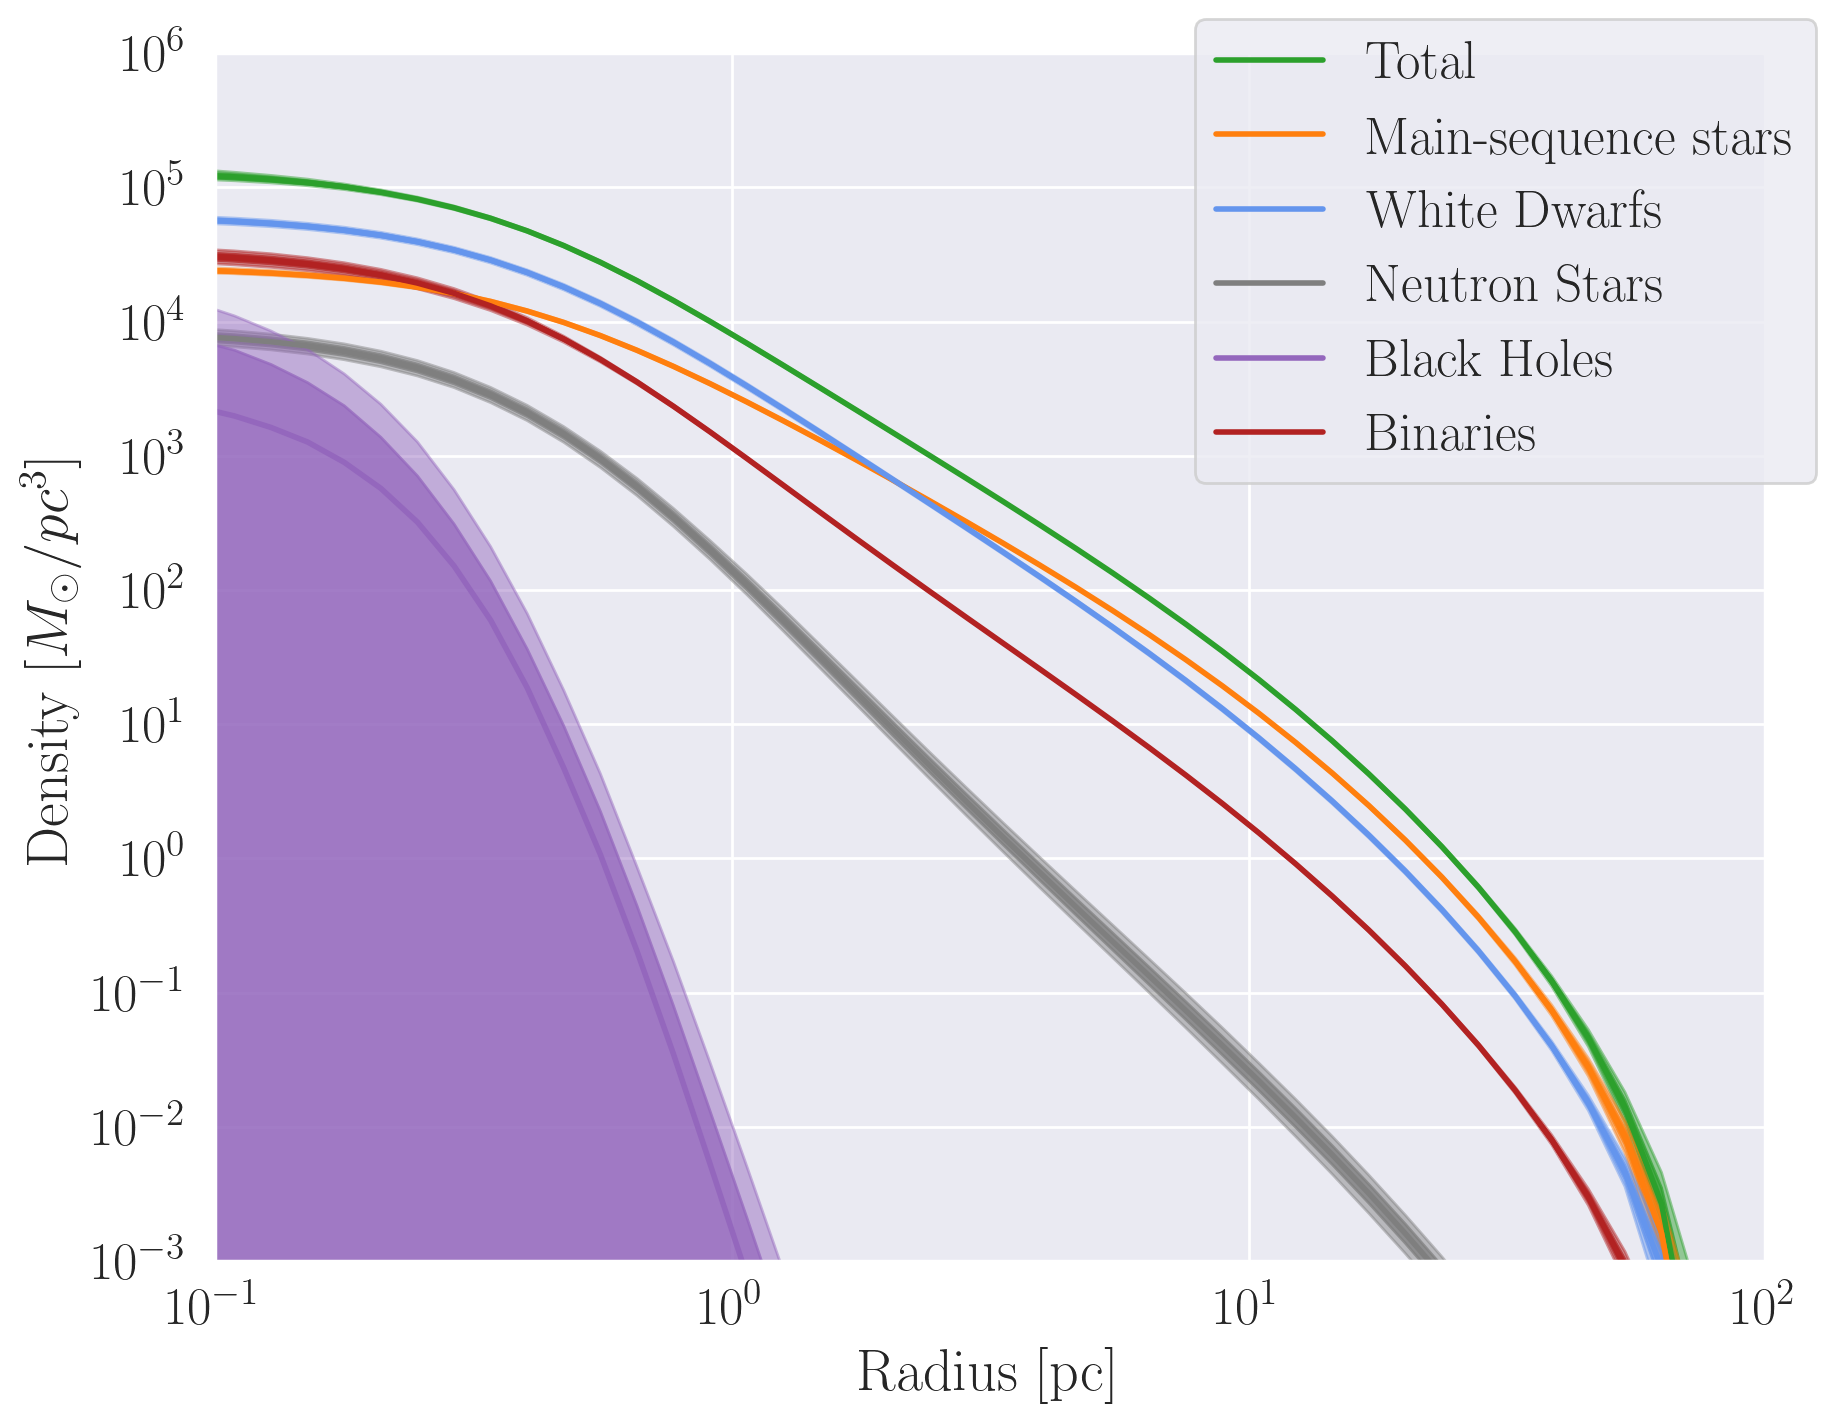
\includegraphics[width=0.8\textwidth]{figures/high_bin_model/density.png}
	\caption{Mass density profiles for the models with a binary fraction of $10\%$}
	\label{fig:highbin_model_densities}
\end{figure}

